\subsection{Interrelación Pregunta - Entrevista}

   \begin{description}
      \item[Definición] En esta interrelación se deja constancia de que una
      entrevista puede estar compuesta de una o varias preguntas.

      \item[Características] La interrelación presenta las siguientes
                             características:

         \begin{itemize}
            \item \textbf{Nombre:} P-Ent
            \item \textbf{Tipo de la interrelación:} El tipo de entidad Pregunta
            es débil por identificación respecto al tipo de entidad Entrevista.
            \item \textbf{Cardinalidad de la interrelación:} N:1
                  \begin{itemize}
                     \item Pregunta: pertenece\_a (1,1)
                     \item Entrevista: tiene (0,n)
                  \end{itemize}
            \item \textbf{Número de atributos:} Ninguno.
         \end{itemize}

      \item[Diagrama] La figura \ref{diagramaP-Ent} muestra el diagrama de la
                      interrelación.

      \item \begin{figure}[!ht]
            \begin{center}
            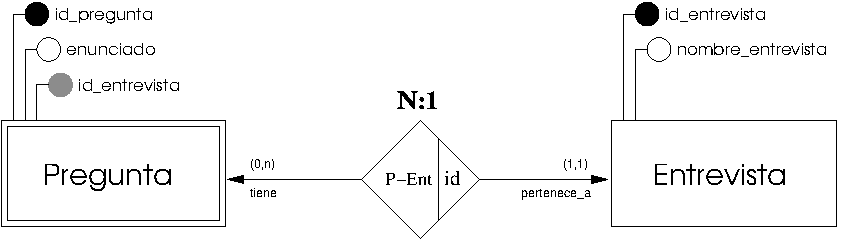
\includegraphics[]{07.Modelo_Entidad-Interrelacion/7.3.Analisis_Interrelaciones/diagramas/P-Ent.pdf}
            \caption{Diagrama de la interrelación P-Ent.}
            \label{diagramaP-Ent}
            \end{center}
         \end{figure}

      \item[Ejemplo práctico del tipo de interrelación]

      \item \begin{center}
            \begin{tabular}{ | r r | }
            \hline
            \multicolumn{2}{ | c | }{\textbf{Tipo de interrelación P-Ent}} \\
            \hline
            \textbf{Pregunta} & \\
            id\_pregunta & 36 \\
            enunciado & Nivel de inglés \\
            id\_entrevista & 24 \\
            \hline
            \textbf{Entrevista} & \\
            id\_entrevista & 77 \\
            nombre\_entrevista & Entrevista idiomas \\
            id\_asesor & 98765432Z \\
            \hline
            \end{tabular}
         \end{center}
   \end{description}
